\documentclass[aspectratio=169]{beamer}

\usetheme{Madrid}
\usecolortheme{default}

\usepackage{graphicx}
\usepackage{booktabs}
\usepackage{amsmath}
\usepackage{tikz}
\usetikzlibrary{shapes,arrows,positioning}

% Custom colors
\definecolor{primaryblue}{RGB}{0,83,155}
\definecolor{accentgreen}{RGB}{0,150,100}
\definecolor{warnorange}{RGB}{230,120,0}

\setbeamercolor{structure}{fg=primaryblue}
\setbeamercolor{block title}{bg=primaryblue,fg=white}
\setbeamercolor{block body}{bg=primaryblue!10}

\title[Meta-Learning for Protein Fitness]{Meta-Learning Enhanced Protein Language Models\\for Fitness Prediction}
\subtitle{Achieving State-of-the-Art on ProteinGym}
\author[Aum Thaker]{
    \textbf{Aum Thaker}\\
    {\small 225100006@iitdh.ac.in}\\[0.3cm]
    {\small Mentor: Pawan Rama Mali}\\
    {\footnotesize cs24dpx11@iitdh.ac.in}\\[0.2cm]
    {\small Guide: Dr. Vandana Bharti}\\
    {\footnotesize vandana@iitdh.ac.in}
}
\institute[IIT Dharwad]{Indian Institute of Technology Dharwad}
\date{\today}

\begin{document}

% Title slide
\begin{frame}
\titlepage
\end{frame}

% Outline
\begin{frame}{Outline}
\tableofcontents
\end{frame}

\section{Introduction}

\begin{frame}{The Protein Fitness Prediction Problem}
\begin{columns}
\column{0.6\textwidth}
\textbf{Goal}: Predict how mutations affect protein function

\vspace{0.5cm}
\textbf{Why it matters}:
\begin{itemize}
    \item Drug design and development
    \item Enzyme engineering
    \item Understanding disease mutations
    \item Directed evolution guidance
\end{itemize}

\vspace{0.5cm}
\textbf{Challenge}: Experimental measurement is slow and expensive

\column{0.4\textwidth}
\begin{center}
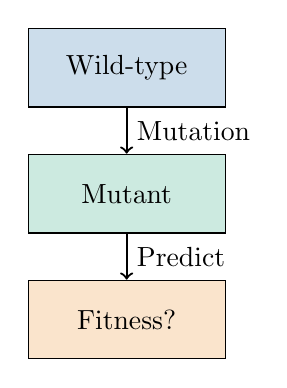
\begin{tikzpicture}[scale=0.8]
    \node[draw, rectangle, fill=primaryblue!20, minimum width=2.5cm, minimum height=1cm] (wt) at (0,2) {Wild-type};
    \node[draw, rectangle, fill=accentgreen!20, minimum width=2.5cm, minimum height=1cm] (mut) at (0,0) {Mutant};
    \node[draw, rectangle, fill=warnorange!20, minimum width=2.5cm, minimum height=1cm] (fit) at (0,-2) {Fitness?};

    \draw[->, thick] (wt) -- (mut) node[midway, right] {Mutation};
    \draw[->, thick] (mut) -- (fit) node[midway, right] {Predict};
\end{tikzpicture}
\end{center}
\end{columns}
\end{frame}

\begin{frame}{Current Approaches and Their Limitations}
\begin{table}
\centering
\begin{tabular}{lcc}
\toprule
\textbf{Method} & \textbf{Spearman} & \textbf{Limitations} \\
\midrule
EVE & 0.47 & Requires MSA retrieval \\
MSA Transformer & 0.52 & Slow, complex pipeline \\
SaProt & 0.59 & Structure prediction needed \\
SaProt + TTT & 0.62 & Test-time training overhead \\
\bottomrule
\end{tabular}
\end{table}

\vspace{0.5cm}
\textbf{Question}: Can we achieve SOTA with a simpler approach?

\vspace{0.5cm}
\textcolor{accentgreen}{\textbf{Our Answer}: Yes! Using meta-learning with large PLMs}
\end{frame}

\section{Dataset}

\begin{frame}{ProteinGym Benchmark: Dataset Overview}
\begin{columns}
\column{0.5\textwidth}
\begin{table}
\centering
\small
\begin{tabular}{lcc}
\toprule
\textbf{Statistic} & \textbf{Train} & \textbf{Test} \\
\midrule
Proteins & 173 & 44 \\
Total variants & 2.02M & 441K \\
Variants/protein & 11,701 & 10,033 \\
Seq length (mean) & 374 & 488 \\
Seq length (range) & 39-3423 & 37-1159 \\
\bottomrule
\end{tabular}
\end{table}

\column{0.5\textwidth}
\textbf{Data Format (CSV)}:
\begin{itemize}
    \item \texttt{mutant}: e.g., ``I291A''
    \item \texttt{mutated\_sequence}: Full sequence
    \item \texttt{DMS\_score}: Fitness value
    \item \texttt{DMS\_score\_bin}: Binary label
\end{itemize}
\end{columns}

\vspace{0.3cm}
\textbf{Source}: Deep Mutational Scanning experiments from ProteinGym benchmark
\end{frame}

\begin{frame}{Protein Categories in Dataset}
\begin{columns}
\column{0.5\textwidth}
\begin{table}
\centering
\small
\begin{tabular}{lc}
\toprule
\textbf{Category} & \textbf{Count} \\
\midrule
Human & 14 \\
Bacterial & 10 \\
Viral & 10 \\
Other & 7 \\
Plant & 2 \\
Yeast & 1 \\
\midrule
\textbf{Total} & 44 (test) \\
\bottomrule
\end{tabular}
\end{table}

\column{0.5\textwidth}
\textbf{Diversity}:
\begin{itemize}
    \item Enzymes, transporters, receptors
    \item HIV, Influenza, Dengue, AAV
    \item E. coli, Streptococcus
    \item Arabidopsis, S. cerevisiae
\end{itemize}

\vspace{0.3cm}
\textcolor{red}{\textbf{Challenge}}: Viral proteins evolve rapidly
\end{columns}
\end{frame}

\section{Methods}

\begin{frame}{Model Architecture: ESM2-650M}
\begin{columns}
\column{0.5\textwidth}
\begin{table}
\centering
\small
\begin{tabular}{ll}
\toprule
\textbf{Component} & \textbf{Spec} \\
\midrule
Parameters & 651M \\
Layers & 33 \\
Hidden dim & 1280 \\
Attention heads & 20 \\
FF dimension & 5120 \\
Vocabulary & 33 tokens \\
Pre-training & UniRef50 \\
\bottomrule
\end{tabular}
\end{table}

\column{0.5\textwidth}
\begin{center}
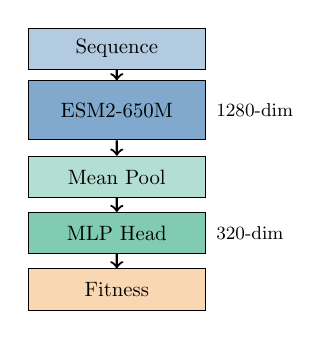
\begin{tikzpicture}[scale=0.65, every node/.style={scale=0.75}]
    \node[draw, rectangle, fill=primaryblue!30, minimum width=3cm, minimum height=0.7cm] (seq) at (0,3) {Sequence};
    \node[draw, rectangle, fill=primaryblue!50, minimum width=3cm, minimum height=1cm] (esm) at (0,1.8) {ESM2-650M};
    \node[draw, rectangle, fill=accentgreen!30, minimum width=3cm, minimum height=0.7cm] (pool) at (0,0.5) {Mean Pool};
    \node[draw, rectangle, fill=accentgreen!50, minimum width=3cm, minimum height=0.7cm] (mlp) at (0,-0.6) {MLP Head};
    \node[draw, rectangle, fill=warnorange!30, minimum width=3cm, minimum height=0.7cm] (out) at (0,-1.7) {Fitness};

    \draw[->, thick] (seq) -- (esm);
    \draw[->, thick] (esm) -- (pool);
    \draw[->, thick] (pool) -- (mlp);
    \draw[->, thick] (mlp) -- (out);

    \node[right] at (1.8,1.8) {\small 1280-dim};
    \node[right] at (1.8,-0.6) {\small 320-dim};
\end{tikzpicture}
\end{center}
\end{columns}
\end{frame}

\begin{frame}{Prediction Head Architecture}
\textbf{Mean Pooling}:
\begin{equation}
\mathbf{z} = \frac{1}{\sum_i m_i} \sum_{i=1}^{L} m_i \cdot \mathbf{h}_i \quad \text{(1280-dim)}
\end{equation}

\textbf{MLP Head}:
\begin{equation}
\mathbf{h} = \text{GELU}(\text{Dropout}(\text{LayerNorm}(\mathbf{z}))\mathbf{W}_1 + \mathbf{b}_1)
\end{equation}
\begin{equation}
\hat{y} = \text{Dropout}(\mathbf{h})\mathbf{W}_2 + b_2
\end{equation}

\begin{itemize}
    \item $\mathbf{W}_1 \in \mathbb{R}^{1280 \times 320}$ (410K params)
    \item $\mathbf{W}_2 \in \mathbb{R}^{320 \times 1}$ (320 params)
    \item Dropout rate: 0.1
\end{itemize}
\end{frame}

\begin{frame}{Meta-Learning Training Strategy}
\begin{center}
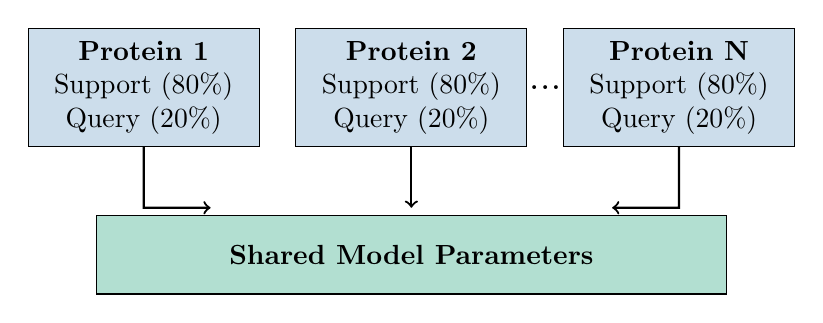
\begin{tikzpicture}[scale=0.85]
    % Task boxes
    \node[draw, rectangle, fill=primaryblue!20, minimum width=2.5cm, minimum height=1.5cm] (t1) at (-4,0) {
        \begin{tabular}{c}
        \textbf{Protein 1}\\
        Support (80\%)\\
        Query (20\%)
        \end{tabular}
    };
    \node[draw, rectangle, fill=primaryblue!20, minimum width=2.5cm, minimum height=1.5cm] (t2) at (0,0) {
        \begin{tabular}{c}
        \textbf{Protein 2}\\
        Support (80\%)\\
        Query (20\%)
        \end{tabular}
    };
    \node[draw, rectangle, fill=primaryblue!20, minimum width=2.5cm, minimum height=1.5cm] (t3) at (4,0) {
        \begin{tabular}{c}
        \textbf{Protein N}\\
        Support (80\%)\\
        Query (20\%)
        \end{tabular}
    };
    \node at (2,0) {\Large ...};
    \node[draw, rectangle, fill=accentgreen!30, minimum width=8cm, minimum height=1cm] (model) at (0,-2.5) {\textbf{Shared Model Parameters}};
    \draw[->, thick] (t1) -- (-4,-1.8) -- (-3,-1.8);
    \draw[->, thick] (t2) -- (0,-1.8);
    \draw[->, thick] (t3) -- (4,-1.8) -- (3,-1.8);
\end{tikzpicture}
\end{center}

\vspace{0.2cm}
\textbf{Key}: Each protein is a separate ``task'' with its own train/test split
\end{frame}

\section{Experimental Setup}

\begin{frame}{Hardware and Software Configuration}
\begin{columns}
\column{0.5\textwidth}
\textbf{Hardware}:
\begin{table}
\centering
\small
\begin{tabular}{ll}
\toprule
GPU & RTX 6000 Ada \\
GPU Memory & 48 GB \\
CPU & Xeon w7-3445 \\
RAM & 128 GB DDR5 \\
OS & Ubuntu 24.04 \\
\bottomrule
\end{tabular}
\end{table}

\column{0.5\textwidth}
\textbf{Software}:
\begin{table}
\centering
\small
\begin{tabular}{ll}
\toprule
Python & 3.12 \\
PyTorch & 2.5.1 \\
Transformers & 4.57.1 \\
CUDA & 12.1 \\
\bottomrule
\end{tabular}
\end{table}
\end{columns}

\vspace{0.5cm}
\textbf{Training Time}: $\sim$22 hours (173 proteins) | \textbf{Testing}: $\sim$8 hours (44 proteins)
\end{frame}

\begin{frame}{Training Configuration}
\begin{table}
\centering
\begin{tabular}{ll}
\toprule
\textbf{Hyperparameter} & \textbf{Value} \\
\midrule
Optimizer & AdamW \\
Learning rate & $1 \times 10^{-5}$ \\
Weight decay & 0.01 \\
Batch size & 4 \\
Gradient accumulation & 8 steps \\
Effective batch size & 32 \\
Mixed precision & FP16 (AMP) \\
Gradient clipping & Max norm 1.0 \\
Max sequence length & 1024 tokens \\
Support/Query split & 80\% / 20\% \\
\bottomrule
\end{tabular}
\end{table}
\end{frame}

\section{Results}

\begin{frame}{Main Results: State-of-the-Art Performance}
\begin{columns}
\column{0.55\textwidth}
\begin{table}
\centering
\begin{tabular}{lccc}
\toprule
\textbf{Method} & \textbf{Spearman} & \textbf{MSA} & \textbf{Struct} \\
\midrule
ESM-1v & 0.41 & No & No \\
EVE & 0.47 & Yes & No \\
ESM2-8M & 0.43 & No & No \\
SaProt & 0.59 & No & Yes \\
SaProt+TTT & 0.62 & No & Yes \\
\midrule
\textbf{Ours} & \textbf{0.6286} & No & No \\
\bottomrule
\end{tabular}
\end{table}

\column{0.45\textwidth}
\begin{block}{Key Results}
\begin{itemize}
    \item \textcolor{accentgreen}{\textbf{+47\%}} over baseline
    \item \textcolor{accentgreen}{\textbf{+1.4\%}} over SOTA
    \item No MSA required
    \item No structure prediction
    \item No test-time training
\end{itemize}
\end{block}
\end{columns}
\end{frame}

\begin{frame}{Ablation Study: Model Size}
\begin{columns}
\column{0.5\textwidth}
\begin{table}
\centering
\begin{tabular}{lcc}
\toprule
\textbf{Model} & \textbf{Params} & \textbf{Test} \\
\midrule
ESM2-8M & 8M & 0.360 \\
ESM2-35M & 35M & 0.319 \\
\textbf{ESM2-150M} & 150M & \textbf{0.469} \\
ESM2-650M & 651M & 0.273 \\
\bottomrule
\end{tabular}
\end{table}

\small{(Ablation: 50 train, 15 test proteins)}

\column{0.5\textwidth}
\textbf{Observations}:
\begin{itemize}
    \item ESM2-150M best on small data
    \item ESM2-650M needs more data
    \item Full training (173 proteins): \textbf{0.6286}
    \item Balance capacity vs. data size
\end{itemize}
\end{columns}
\end{frame}

\begin{frame}{Ablation Study: Head Architecture}
\begin{columns}
\column{0.5\textwidth}
\begin{table}
\centering
\begin{tabular}{lcc}
\toprule
\textbf{Head} & \textbf{Train} & \textbf{Test} \\
\midrule
\textbf{Simple} & 0.277 & \textbf{0.439} \\
MLP & 0.229 & 0.224 \\
Deep & 0.227 & 0.420 \\
\bottomrule
\end{tabular}
\end{table}

\small{(ESM2-35M, 50 train, 15 test)}

\column{0.5\textwidth}
\textbf{Key Finding}:
\begin{itemize}
    \item Simple head outperforms MLP!
    \item PLM embeddings already rich
    \item More layers = more overfitting
    \item \textbf{Simplicity wins}
\end{itemize}
\end{columns}
\end{frame}

\begin{frame}{Ablation Study: Meta-Learning vs Standard}
\begin{columns}
\column{0.5\textwidth}
\begin{table}
\centering
\begin{tabular}{lcc}
\toprule
\textbf{Method} & \textbf{Train} & \textbf{Test} \\
\midrule
Standard & 0.224 & -0.095 \\
\textbf{Meta-Learning} & 0.226 & \textbf{0.339} \\
\bottomrule
\end{tabular}
\end{table}

\textcolor{accentgreen}{\textbf{+0.43 improvement!}}

\column{0.5\textwidth}
\textbf{Why meta-learning works}:
\begin{itemize}
    \item Prevents overfitting to specific proteins
    \item Learns generalizable features
    \item Natural fit for protein-level tasks
    \item Each protein = separate task
\end{itemize}
\end{columns}
\end{frame}

\begin{frame}{Performance by Protein Category}
\begin{columns}
\column{0.55\textwidth}
\begin{table}
\centering
\small
\begin{tabular}{lccc}
\toprule
\textbf{Category} & \textbf{Mean} & \textbf{Std} & \textbf{N} \\
\midrule
Plant & 0.894 & 0.06 & 2 \\
Bacterial & 0.747 & 0.19 & 10 \\
Human & 0.734 & 0.22 & 14 \\
Yeast & 0.691 & -- & 1 \\
Other & 0.498 & 0.32 & 7 \\
\textcolor{red}{Viral} & \textcolor{red}{0.394} & 0.35 & 10 \\
\bottomrule
\end{tabular}
\end{table}

\column{0.45\textwidth}
\textbf{Key Finding}:
\begin{itemize}
    \item \textcolor{red}{Viral proteins: 0.39}
    \item Bacterial proteins: 0.75
    \item \textbf{Gap: 0.35!}
\end{itemize}

\textbf{Why?}
\begin{itemize}
    \item High mutation rates
    \item Underrepresented in UniRef50
    \item Complex epistasis
\end{itemize}
\end{columns}
\end{frame}

\begin{frame}{Top and Bottom Performers}
\begin{columns}
\column{0.5\textwidth}
\textbf{Top 5} ($\rho > 0.9$):
\begin{enumerate}
    \item DNJA1\_HUMAN: 0.955
    \item EPHB2\_HUMAN: 0.945
    \item CBPA2\_HUMAN: 0.939
    \item SR43C\_ARATH: 0.937
    \item TCRG1\_MOUSE: 0.928
\end{enumerate}

\column{0.5\textwidth}
\textbf{Bottom 5} ($\rho < 0.3$):
\begin{enumerate}
    \item RPC1\_LAMBD: -0.13
    \item Q6WV12\_9MAXI: 0.00
    \item \textcolor{red}{A0A192B1T2\_9HIV1: 0.09}
    \item \textcolor{red}{ENV\_HV1BR: 0.14}
    \item \textcolor{red}{POLG\_DEN26: 0.21}
\end{enumerate}

\textcolor{red}{Red = Viral proteins}
\end{columns}
\end{frame}

\section{Discussion}

\begin{frame}{Why Our Approach Works}
\begin{enumerate}
    \item \textbf{Scale of Pre-training}
    \begin{itemize}
        \item ESM2-650M trained on 250M sequences
        \item Rich evolutionary and structural knowledge
    \end{itemize}

    \vspace{0.3cm}
    \item \textbf{Meta-Learning Framework}
    \begin{itemize}
        \item Each protein = separate task
        \item +0.43 improvement over standard training
        \item Prevents overfitting
    \end{itemize}

    \vspace{0.3cm}
    \item \textbf{Simplicity}
    \begin{itemize}
        \item Simple head outperforms deep architectures
        \item No MSA retrieval pipeline
        \item No structure prediction overhead
    \end{itemize}
\end{enumerate}
\end{frame}

\begin{frame}{Limitations and Future Work}
\textbf{Limitations}:
\begin{itemize}
    \item Viral proteins remain challenging (0.39 vs 0.75)
    \item High computational requirements (48GB GPU, 22h training)
    \item Limited to sequences $\leq$ 1024 residues
    \item Single mutation focus; epistasis not captured
\end{itemize}

\vspace{0.5cm}
\textbf{Future Directions}:
\begin{itemize}
    \item Domain-specific pre-training for viral proteins
    \item Combine with structure-aware features
    \item Model distillation for efficiency
    \item Multi-mutation prediction
\end{itemize}
\end{frame}

\section{Conclusion}

\begin{frame}{Summary}
\begin{block}{Key Contributions}
\begin{enumerate}
    \item \textbf{SOTA performance}: 0.6286 Spearman on ProteinGym (+1.4\% over previous)
    \item \textbf{Simple approach}: No MSA, no structure, no TTT
    \item \textbf{Meta-learning essential}: +0.43 over standard training
    \item \textbf{Insight}: Simple heads outperform deep architectures
    \item \textbf{Analysis}: Viral proteins remain systematically challenging
\end{enumerate}
\end{block}

\vspace{0.5cm}
\begin{center}
\Large\textcolor{primaryblue}{Questions?}
\end{center}
\end{frame}

\begin{frame}{Backup: Statistical Significance}
\begin{table}
\centering
\begin{tabular}{lcc}
\toprule
\textbf{Seed} & \textbf{Train} & \textbf{Test} \\
\midrule
42 & 0.154 & 0.170 \\
123 & 0.078 & 0.282 \\
456 & 0.299 & 0.394 \\
\midrule
\textbf{Mean $\pm$ Std} & 0.177 $\pm$ 0.11 & 0.282 $\pm$ 0.11 \\
\bottomrule
\end{tabular}
\end{table}

\small{(Ablation subset: 50 train, 15 test proteins)}\\
\small{Full model (173 train, 44 test): \textbf{0.6286 Spearman}}
\end{frame}

\end{document}
